\section{Teorija asinhronega prenosa in obdelave podatkov} \label{a}


\subsection{Osnove / Hitrostna neodvisnost} \label{b}

Naredimo model asinhronih vezji, da bolje razumemo kako delujejo. Predstavljajmo si vezje vrat, povezanih med seboj. Vsaka vrata imajo vhodne in izhodne signale. Ko vhod vrat diktira spremembo izhoda postanejo vrata aktivna. Po neznanem časovnem zamiku se spremeni tudi izhod. Zanimivo je, kar se zgodi na izhodu vrat. Vrata ki imajo na vhodu izhodini signal naše originalnih vrat imajo tri opcije.
Lahko sprememba vhoda ne spremeni izhoda.
Lahko sprememba vhoda ne povzroči spremembe izhoda.
Lahko pa so bila vrata aktivna, a zaradi spremembe izhoda sedaj niso več aktivna.

Vezja, kjer se zadnji kriterij nikoli ne zgodi so hitrostno neodvisna.

Moramo poskrbeti da si signali sledijo v urejenem zaporedju.


Poglejmo katere predpostavke uporabljamo:

Hitrostno neodvisna vezja imajo neznane zakasnitve v vratih in nimajo zakasnitev v žicah. To žal ni zelo realno.

Vezja, ki so neodvisna na zakasnitve imajo neznane zakasnitve v žicah in vratih, tu ne predpostavimo nič, ampak takih vezji je zelo malo. Citat

Srednja pot je kvazi zakasnitvena neodvisnost, kjer imamo določene predpostavke, o zakasnitvah v žicah.






\subsection{Osnovna vezja} \label{b}
Če želimo načrtovati asinhrona vezja je torej potrebno sinhronizirati vse signale z najpočasnejšim. Poglejmo si kako lahko to dosežemo.

\subsubsection{Muller C element} \label{c}
Muller C element je osnovni element sinhronizacije dveh signalov. Ima dva vhoda, izhod se spremeni, ko sta oba vhoda enaka.

\begin{figure}
	\centering
	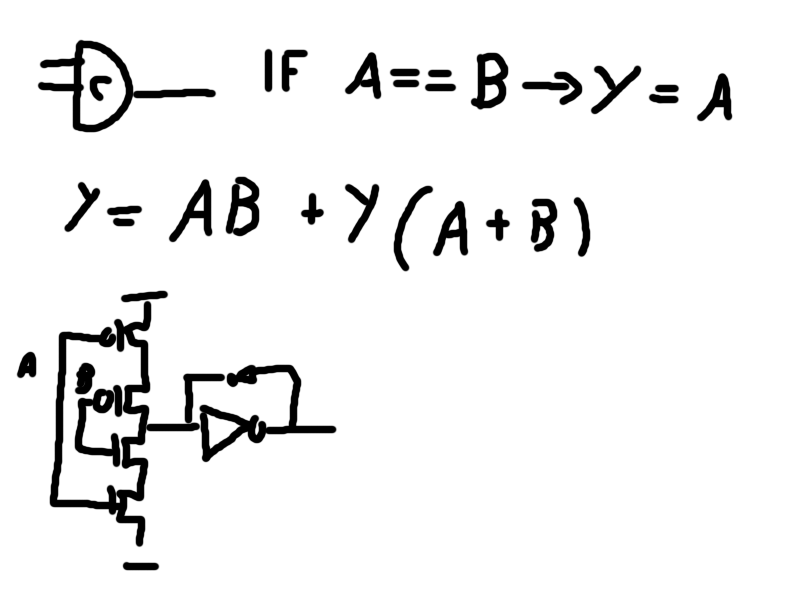
\includegraphics[width=0.7\linewidth]{slike/C_Element}
	\caption{}
	\label{fig:celement}
\end{figure}

Poglejmo si kako tak element sinhronizira dva signala:

Imamo dve povratni zanki, vsaka z različno zakasnitvjo, kateri želimo sinhronizirati.

\begin{figure}
	\centering
	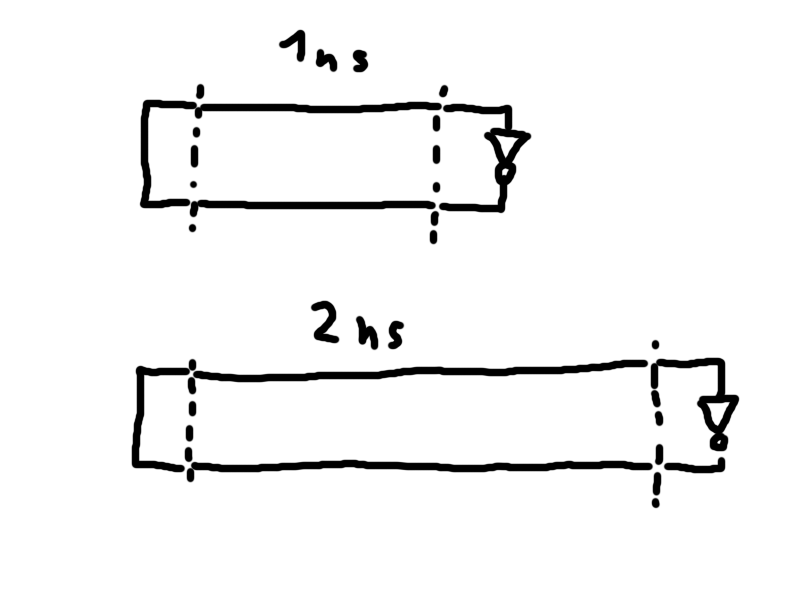
\includegraphics[width=0.7\linewidth]{slike/dly1}
	\caption{}
	\label{fig:celement}
\end{figure}

Če ustvarimo prek C elementa skupno povratno zanko, mora hirejši vedno čakati počasnejšega, torej sta sinhronizirana.

\begin{figure}
	\centering
	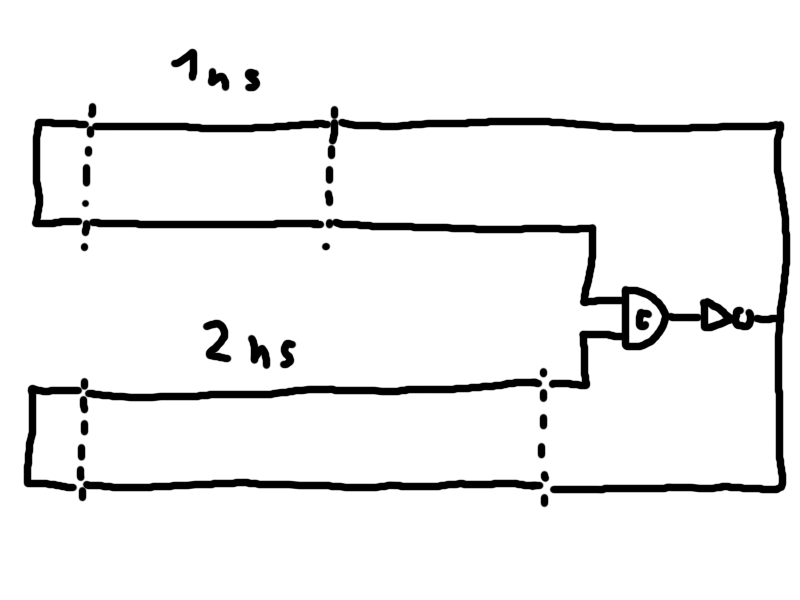
\includegraphics[width=0.7\linewidth]{slike/dly2}
	\caption{}
	\label{fig:celement}
\end{figure}

Trivialno lahko sinhroniziramo poljubno število povratnih zank.

\begin{figure}
	\centering
	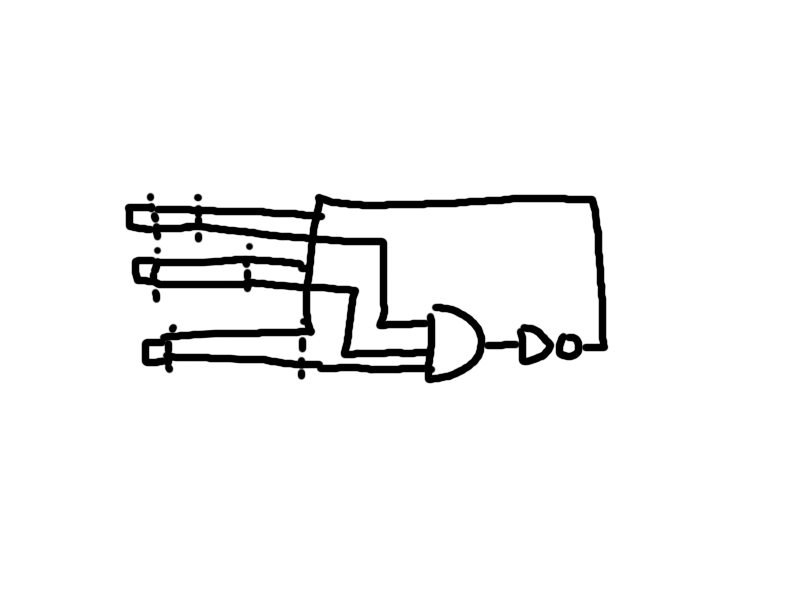
\includegraphics[width=0.7\linewidth]{slike/dly3}
	\caption{}
	\label{fig:celement}
\end{figure}

To lahko razumemo kot vzporedno vezavo oscilatorjev, kjer je skupna perioda, perioda najdaljše povratne zanke. 
Lahko pa vežemo oscilatorje tudi vzporedno na sledeči način:

%Inverter na napacni strani

\begin{figure}
	\centering
	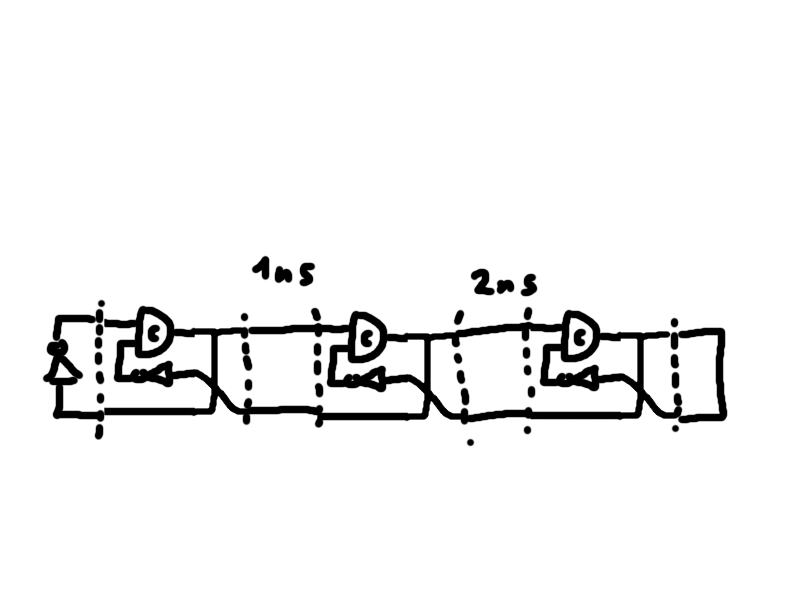
\includegraphics[width=0.7\linewidth]{slike/dly4}
	\caption{}
	\label{fig:celement}
\end{figure}

Tu povratne zanke prepletemo med seboj. Vsako povratno zanko sprožijo njeni sosedje. V tem primeru prva zanka sproži drugo. Ko druga konča ponovno sporži prvo.

Tak vzorec lahko nadaljujemo poljubno dolgo.
\begin{figure}
	\centering
	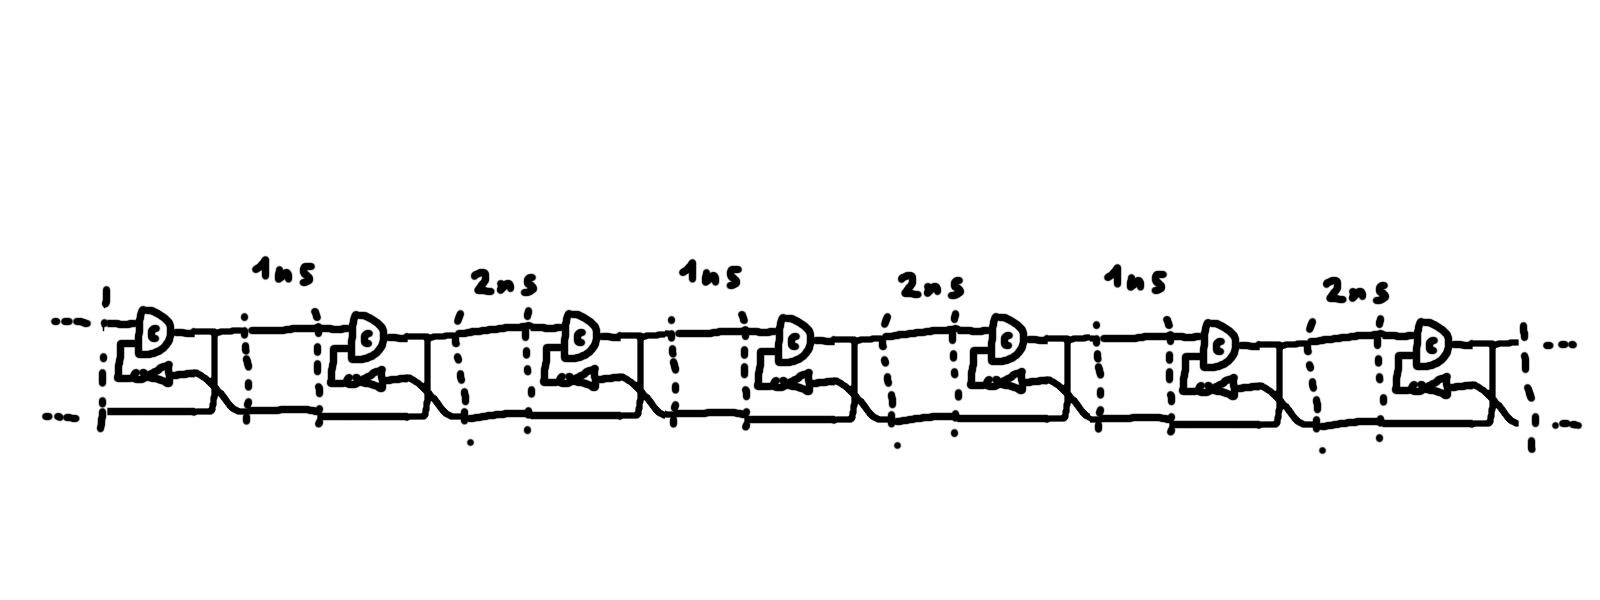
\includegraphics[width=0.7\linewidth]{slike/dly5}
	\caption{}
	\label{fig:celement}
\end{figure}


\subsubsection{Cevovodi} \label{c}

Linija iz knjige:
A register may input and store a new data token from its predecessor if
its successor has input and stored the data token that the register was pre-
viously holding.

Če pogledamo dano vezje lahko vidimo, da deluje kot 1-biten FIFO. Podatki se nalagajo noter in črpajo ven. Temu konstruktu se reče Mulerjev cevovod, in je osnova vseh asinhronih vezji.

Lahko naredimo tudi obroče, Ali več sklenjenih obročov...

Osnovna celica cevovoda je..., če pogledamo logične funkcije: ..., To lahko izvedemo tudi na druge načine.

\subsubsection{Podatkovno procesiranje} \label{c}

Sedaj imamo cevovode, želimo med stopnjami cevovoda procesirati podatke. Dva načina:
\begin{itemize}
	\item vzporedno imamo default logiko - Bundlede data
	\item Vzporedni sklopljeni cevovodi
\end{itemize}
 
 Vzporedno logika, timing assumptions, delays kako prožit latche, samo pol jih ima naenkrat noter data, isto kot v sinhronih vezjih.
 
 Vzporedni cevovdi, kako sklopit, kako procesirat podatke ect...
 
%I love U <3

%
%A code (I ,C) is called delay-insensitive when :MATH @ dicodes:that is, when no code word is contained in another code word
%



\section{Protokoli} \label{a}
Zgornja načina plus 2/4 phase.
\begin{itemize}
	\item 2phase hitrejsi, ampak rabimo feedback da vemo kdaj smo done
	\item 4phase preprostejši več komunikacije
\end{itemize}

Kartezični produkt:

\subsection{4-Phase dual rail} \label{b}
Karl Fant, dve žici na bit ect

\subsection{4-bundled data} \label{b}
lepa logika, ampak potrebujemo zakasnitve (lahko predvidimo zakasnitve)

\subsection{2-Phase dual rail} \label{b}
Ta magisterska

\subsection{2-bundled data} \label{b}
Micropipelines ect.


\section{Podatkovni potek} \label{a}
Podatki se pretakajo po asinhronih vezjih kot valovi. v eno smer gre data, v drugo gre ACK. Vedno moramo kontrolirati število podatkovnih valov v vezju ect.
To lahko gledamo kot graf po katerem se pretekajo tokeni. 

Osnova igre ect:

Drugače za 2 phase kot za 4 phase:

\subsection{2phase} \label{b}
Najmanj 2 v ciklu poljubno število, inicializacija. Vrsta grafa, za to

\subsection{4phase} \label{b}
Najmanj 3 v ciklu sodo število, inicializacija. Vrsta grafa, za to

